\chapter{Introduction}
\section{Background}
Urban water challenge increases as the cities grow larger. The World Bank estimates that the urban population in worldwide will double by 2050---with serious implications of escalating water demands in cities by 50--70 precent \citep{theworldbankCircularEconomyOpportunity2021}. The amount, distribution, and quality of the available fresh water in urban water cycle has largely been affected by the global climate change. The report from \citep{unicefURBANWATERSCARCITY2021} points out that one in four cities are facing challegnes to supply adequate water to inhabitants, the situation is even worse in cities from developing wrold. The rise of urban water usage will generate more wastewater, thus, the conversion of municipal/industrial wastewater into reusable water is drawing much attentions over the years. Reuse water increases the water availability by substituting the use of freshwater on non-potable (drinkable) uses for agricultural irrigation, industrial, and urban water reuses, etc. The alternative reuse water can supply many activities and save drinking water for other purposes elsewhere \citep{adewumiTreatedWastewaterReuse2010}.

The construction of reclaimed water facilites often require a huge amount of capital investment. Upgrading available wastewater treatment plants with the reuse water treatment facilities is an economic solution which accompanied with the benefits of the potential of realizing resource recovery (e.g., nitrogen and phosphorus recovery) \citep{maryamWastewaterReclamationReuse2019,kehreinCriticalReviewResource2020}. The primary concern of reusing treated wastewater is the the potential risks caused to the public health. Under unexpected circumstances, it is possible for the reclaimed water facilites to produce unqualified reclaimed water, which is harmful to the living beings (i.e., as reuse water is ingested directly or through irrigated crops) and irrigated soil \citep{adewumiTreatedWastewaterReuse2010}. In Hong Kong, reclaimed water quality is regulated with up to 10 or more water quality parameters, and any parameters fail to meet the standard will lead to disqualification. The common practice for controlling the treated water quality is achieved through water quality control strategy. The market controllers have evoled from a simple on-off logic controller called Programmable Logic Controller (PLC), to a more advanced multi-step response controller called proportional-integral-derivative (PID), and finally to the controller consists of machine learning models. 

%controller can refer to the entire system or the mathematical equations

The deployment of machine learning models in the water quality controllers for assisting water quality control strategy is a ground-breaking application. Many research papers have proposed various machine learning models for replacing the PLC and PID controllers, and demonstrated the benefits machine learning have brought. From the study of \citep{librantzArtificialNeuralNetworks2018}, the disinfection process in a drinking water treatment plant, a PID and machine learning based controller were depolyed to compare the operational costs of meeting the chlorine concentration set-point (i.e., the controller is set to increase or decrease the chlorine dosage until a specific concentration is reached). The results showed that Artificial Nerual Network based model has a more satisfied cost reduction in a chlorination dosing control system comapred to PID controller. Another reseach finding suggests using a Support Vector Regression (SVR) model as the controller required less time in reaching the set-point concentration of free chlorine residual compared to PID controller in both simulation and experimental conditions \citet{wangModelPredictiveControl2020}.

The superior performance of machine learning models comes from the tranining of high-quality datasets with good amount of data and data which can fairly represents the dynamic of the system. Previous work has only focused on how the models were trained by the dataset and the performance comparisons between models and PID controllers in water quality control. This raises many questions such as in the senarios when the amount of data is insufficient in length or types (i.e., only a few variable such as pH values or chlorine concentration are available), or the collected data is in poor quality (i.e., missing values or exists extreme values). Although a few papers have discussion the use of data pre-processing methods for removing the noise in raw dataset using data smoothing filters \citep{chengForecastingWastewaterTreatment2020}, or creating new features in addition to the raw dataset \citep{mamandipoorMonitoringDetectingFaults2020}, the influence of data pre-processing methods on the model outputs were not revealed.

Machine learning models for water quality control have two main types of algorithms, regression and classification. The former provides forecasting results of specific values, while the latter provides a decision of yes or no (i.e., 1 or 0). Regression model is also called forecasting models, which play an important roles in water quality control in drinking water treatment plants (DTPs) 
and wastewater treatment plants (WWTPs). The need of using forecasting models are becuase the unpredictable nature of water quality, and the treatment operations are subjected to the change of water quality to produce effluent complied the government regulation \cite{chenAssessingWastewaterReclamation2003}. In the reclaimed water system in Shek Wu Hui Effluent Polish Plant (SWHEPP), forecasting models are needed for the effluent treatment management and operation. However, only limited online sensors are availabe onsite. Despite the access to limisted data for model training, it's still possible to train a forecasting model with one input, which is also called a self-prediction model. In this study, we will attempt to build machine learing models for forecasting water quality patameter in reclaimed water. Meanwhile, the issue of insufficienct data in quantity will be addressed with data pre-processing methods. 

%6. Explaining the key terminology in your field

%Explaining how you will use terminology and acronyms in your paper



%paragraph 1 Forecasting models play an important role in water quality control in DTPs and WWTPs.
%paragraph 2 Water reclamation-why is it a good choice for solving urban water scarcity
%paragraph 3 Decision-making processing-how does this help water reclamation
%paragraph 4 Deep learning model to replace fuzzy supervisor and machine learning models-the need of using it
%AI technologies have been successfully applied to different DWT processes, such as the prediction of the coagulant 
%dosage, discrimination of the DBP formation potential, advanced control of membrane fouling, membrane preparation 
%and optimization, and water quality prediction. \cite{liRecentAdvancesArtificial2021}


%\begin{figure}[!t]
%   \centering
%   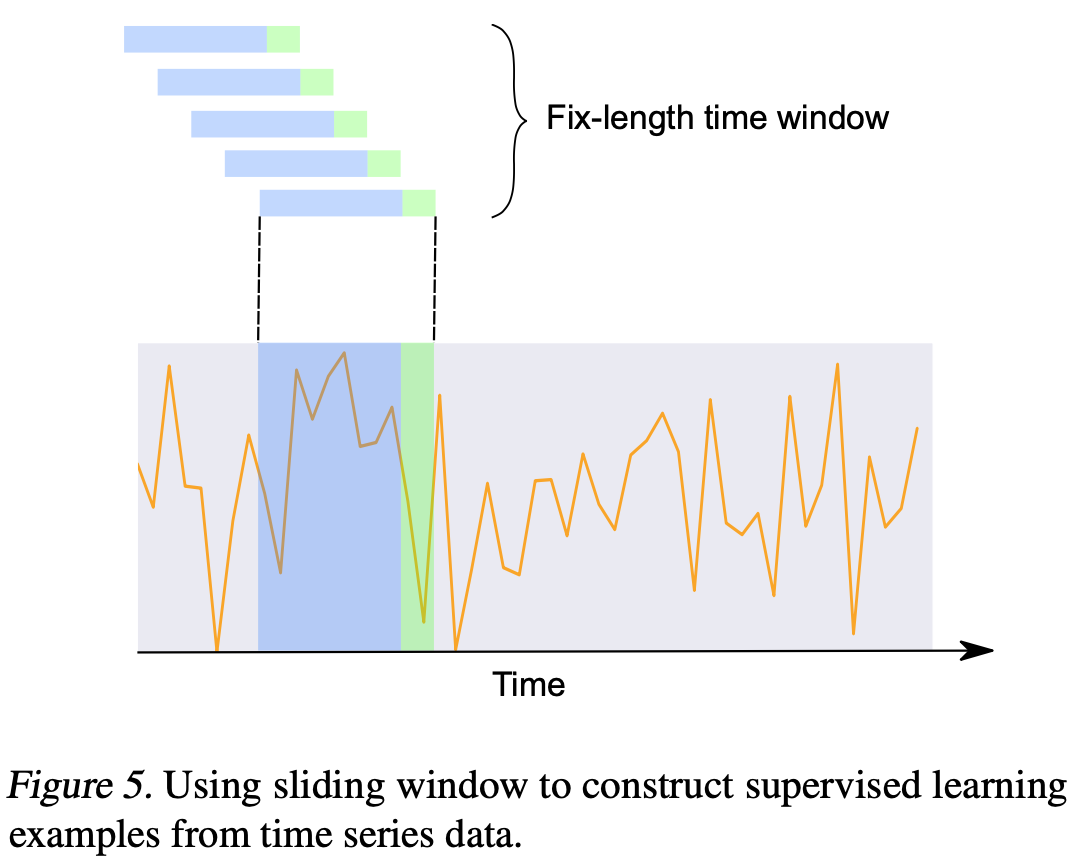
\includegraphics[width=0.75\columnwidth]{imgs/fix-length-time-window.png}
%   \caption{The network structure for the actor-evaluation estimation. It is a combination of convolutional networks for feature extraction and fullyconnected layers for policy learning. They have been separately proven to be effective in our previous works.}
%   \label{fig:ob_network_structure}
%\end{figure}

\section{Objectives}
\noindent
The specific objectives of this thesis work are:\\
%should be investigate the effluent water quality in SWHEPP?
(1) To build baseline univariate forecasting models using machine learning and deep learning models.\\
(2) To develop data preprocessing methods for enhancing model forecasting performance.\\
(3) To extract features and hidden relations of water parameters in MBR effluent by analyzing the wastewater collected upstream of the WWTPs.\\
(4) To develop methods for improving performance of forecasting models using the hidden features and relations of the water parameters.

\section{Organization of the thesis}
In Chapter 1, “Introduction”, the background information, objectives and organization of the thesis were presented.

Chapter 2, “Literature Review”, provides the overview of water quality process controls, the reviews cover the water treatment plant, wastewater treatment plant, and in reclaimed water system.

In Chapter 3, “Materials and Methods”, the instruments for ammonia and colour data collection, programming environment, and data preparation methods were summarized. The processes of the formulation of extra features for training forecasting models were illustrated.

In Chapter 4, “Results and discussion”, the performance of machine learning and deep learning models were compared. Forecasting models trained by different data pre-processing methods and the effect of feature engineering were both compared with the baseline model performance. 

In Chapter 5, “Conclusions and Recommendations”, the findings obtained from this thesis work were summarized and the possible future studies were recommended.